\doublespacing

In the Monte Carlo (MC) code, the \texttt{RANGE} value determines the ratio with which the steps of the Metropolis-Hastings algorithm (see Sec.~\ref{ssec:compFerm}) are accepted, which is ideally $\approx50\%$ \cite{jain}. We used Hernandez's data from Appendix A of Ref. \cite{uriel} to fit the parameters for the \texttt{RANGE} values that correspond to a $50\%$ acceptance ratio as a function of the number of electrons $N$ at filling factor $\nu=1/3$ in the lowest Landau level (LLL). In our computational experiments, these \texttt{RANGE} values seemed to produce similar results for $\nu\in\{2/5,3/7,4/9,5/11,...\}$, but further study needs to be done to determine quantitatively how accurate this formula is at other filling factors. The equation of best fit,
\begin{equation}\label{range}
\texttt{RANGE}(N)=1.211910N^{−1.419258}+0.018149,
\end{equation}
is plotted along with the data from Ref. \cite{uriel} in Fig. \ref{fig:range_vs_n}.

\begin{figure}[H]
\begin{center}
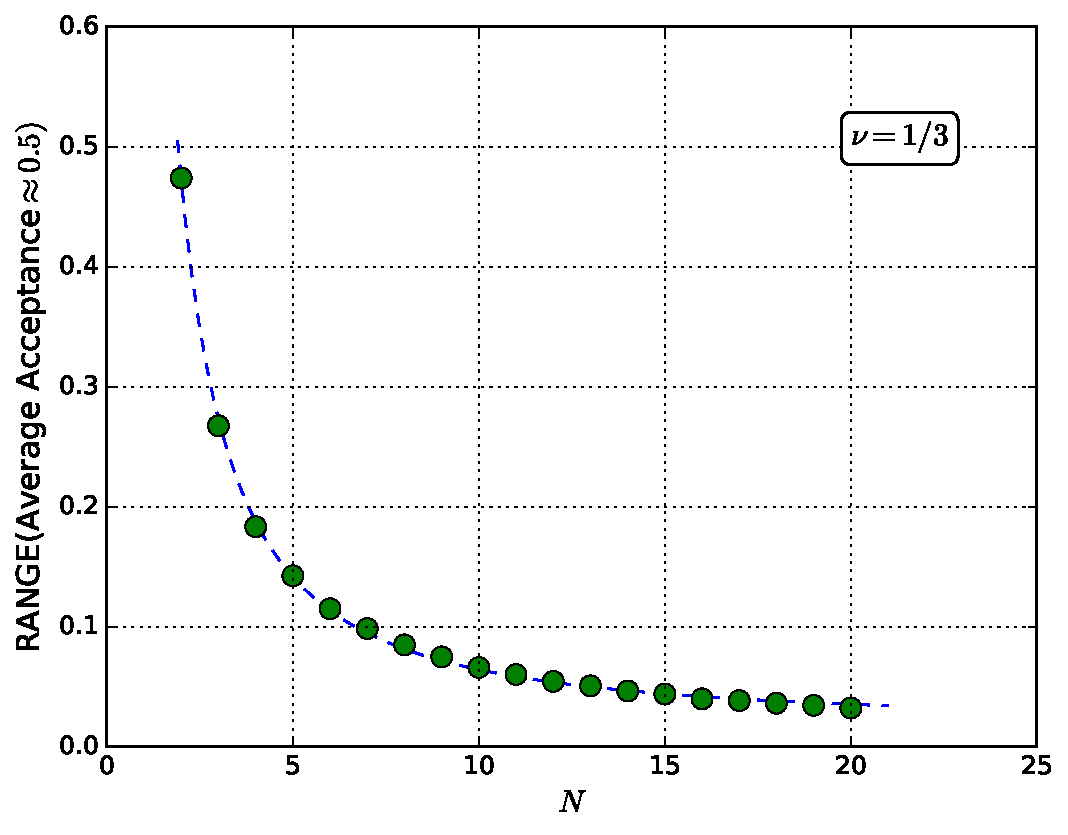
\includegraphics[width=10cm, angle=0]{ThesisCSULBLatexTemplate/figures/range_vs_n.pdf}
\caption[Monte Carlo \texttt{RANGE} values.]{Monte Carlo \texttt{RANGE} values. The equation of best fit for the \textt{RANGE} values that produced a 50\% acceptance ratio in the Monte Carlo code are plotted as a function of the number of electrons $N$ at filling factor $\nu=1/3$ in the LLL.}
\label{fig:range_vs_n} 
\end{center}
\end{figure}

\singlespacing